\chapter{Details about the Angle Resolved Photoemission Experiments}	% *NOT* \OnePageChapter

\section{Experimental Details of the ARPES Experimentsl}
We use a multi-pass Ti:Sapphire laser system to generate 28 fs pulses at a wavelength of 780 nm (1.6 eV) with pulse energy of 2.0 mJ and a repetition rate of 4 kHz. Most of the laser energy (95\%) is used for high-harmonic generation (HHG), while a small portion (5\%) is used to excite the sample as the pump. To generate HHG, we send 95\% of the laser power into a 200 $\mu$m thick $\beta$-phase barium borate (BBO) crystal, which produces pulses at a wavelength of $\approx$390 nm with pulse energy $\approx$ 0.3 mJ. The residual 780 nm light is removed from the beam path using two dichroic mirrors after the BBO. The 390 nm light is then focused using a lens with 50 cm focal distance into a 1-cm-long capillary waveguide. The waveguide has an inner diameter of 150 $\mu$m and is filled with Xe at a pressure of $\approx$20 Torr or Kr at a pressure of $\approx$60 Torr. The HHG beam is focused onto the nickel sample in the UHV chamber using a toroidal BK7 mirror to a spot size of $\approx$100 μm in full width of half maximum (FWHM). Any residual driving laser light is blocked by a 200 nm thick polycrystalline Al filter. The excited photoelectrons are collected by a hemispherical electron analyzer. The energy resolution is calibrated using the photoemission spectrum from a polycrystalline Cu at the room temperature and yields $\approx$160 meV. For ARPES, the atomically clean Ni(111) surface is obtained in-situ using repeated cycles of Argon ion sputtering (0.5 keV) at room temperature, followed by annealing to 900 K for 15 minutes.

The linearly polarized 780 nm pump beam is recombined collinearly with the HHG beam using an annular silver mirror and focused onto the sample surface. The pump fluence is varied by the combination of a half waveplate and a polarizer, as shown in Fig. \ref{fig: NiSIfig1}A. The pulse durations of the pump-probe experiment is directly measured in-situ using the laser-assisted photoemission (LAPE) method. In the LAPE measurement, p-polarized pump light is focused onto the sample surface. When the pump pulse temporally overlaps with the HHG-probe pulse, a side band can be clearly observed at an energy 1.6 eV away from the main photoemission peak, which allows us to extract the cross-correlation of the pump and probe pulses. The side band intensity as a function of td obtained from LAPE measurement is shown in fig. S1B. We note that in order to avoid the influence of LAPE signals on our measurements of ultrafast charge and exchanging splitting dynamics, we switch to s-polarized IR pump in the other two measurements.

\section{Dynamics of electron temperature}
The photoelectron spectra of Ni(111) along  direction are measured using $\approx$16 eV photons from HHG. After Shirley background subtraction (43), the photoemission intensity across $E_{F}$ can be described by the Fermi-Dirac (FD) distribution multiplied by the density of states of the material. In order to extract the time-dependent electron temperature ($T_e$), we fit the photoemission intensity (I) integrated from k$\/\/ \approx$ 0.85 $\AA^{-1}$  to k$\/\/ \approx$ 1.3 $\AA^{-1}$ as shown in Fig. \ref{fig: NiSIfig2}A to the function,
\begin{equation}
I(t_{d})=\{A(t_d)\times FD[E_F(t_d),T_e(t_d)]\times DOS[E_F(t_d)-E_B,\sigma_L]\}\times\textit{Gauss}(\sigma_G)
\label{eqn:S1}
\end{equation}
where A is the amplitude parameter, FD the Fermi-Dirac function. DOS in Eq. \ref{eqn:S1} is the density-of-states function, modeled as a Lorentzian peak with a peak center at $E_F$-$E_B$ and a peak width of $\sigma_L$. Here, $E_B$ is the binding energy of the state. The function is finally convolved with a Gaussian function (Gauss) with a width $\sigma_G$, which represents the energy resolution of $\approx$160 meV in our experiments. The fitting error of the photoemission intensity to Eq. \ref{eqn:S1} is defined as $\sigma_{fit}$.

We note that with pump fluences F>2 mJ/$cm^2$, the space charge effects caused by surface charging and multi-photon photoemission induced by the IR pump laser are inevitable, and induce time-dependent energy shifts of the photoemission spectra in the Tr-ARPES experiments(45). At the same time, because we are only interested in the photoemission intensity within $\approx$1 eV across EF, the space-charge induced energy shifts in this small energy window can be assumed to be an energy-independent constant. As a result, in Eq. \ref{eqn:S1}, we model the Fermi energy $E_F$ as a time-dependent parameter, while the binding energy of the state ($E_B$) is a time independent parameter. Because the electron temperature $T_e$ is determined by the slope of the FD function across $E_F$, this fact allows us to mostly decouple $T_e$ from the space-charge induced energy shifts in the fitting procedure.

When fitting the photoemission intensities at different td to eq. S1, we first determine the time independent parameters ($E_B$, $\sigma_L$) with the spectrum obtained at $t_d$ before the pump-probe time zero (e.g. $t_d$ = -500 fs). Then we can fix these parameters in the following fitting procedures for the other $t_d$. Typically, $E_B \approx$ 0.15 eV and $\sigma_L \approx$ 0.4 eV are used for all the data sets. The time dependent parameters $E_F$ and $T_e$ can be reliably extracted using the fitting procedure described above. The fitting results for F $\approx$ 6 mJ/cm2 at $t_d$ = -500 fs and 24 fs are shown as an example in Fig. \ref{fig: NiSIfig2}B and C. The extracted values of $E_F$ also allow us to compensate the pump-induced space charge effect by assuming EF is constant after pump excitation. Indeed, the chemical potential of the majority and minority electrons can be different and shift as the electron temperature varies, but the amount of energy shift is only several meV even with the electron temperature elevated by $\approx$ 2000 K(46). The photoemission intensity at different td are plotted without the space-charge correction in Fig. \ref{fig: NiSIfig2}D and with the correction in Fig. \ref{fig: NiSIfig2}E.

\begin{figure}[htbp]
	\begin{center}
		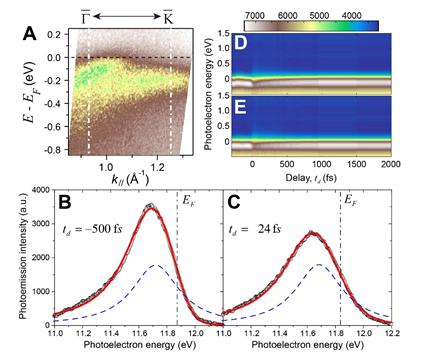
\includegraphics[width=150mm]{figs/NiFigS2}
	\end{center}
	\caption{Electron temperature fitting. (A) Photoemission spectrum of Ni(111) excited by 16 eV HHG photons at room temperature. The white dash-dotted lines represent the momentum range for the photoemission intensity in the analysis for the transient electron temperature. (B) and (C) Photoemission intensity and fitting results at $t_d$ = -500 fs and $t_d$ = 24 fs for F $\approx$ 6 mJ/cm2. The red solid lines are the fitting results using Eq. \ref{eqn:S1} and the blue dashed lines represent the DOS function used in the fitting. The black dashed-dot lines are the Fermi energy obtained from the fitting. (D) Photoemission intensity as a function of pump-probe time delay from the raw experimental data. (E) Same as (D), but the $E_F$ shifts due to pump-induced space charge effects are corrected. }
	\label{fig: NiSIfig2}
\end{figure}

Moreover, the energy resolution of $\approx$160 meV in our experiments places a lower limit on the electron temperature we can extracted from the experiments and this limit has to be considered as part of the errors in our data analysis. In order to determine how much the errors from the energy resolution contribute, we model a FD distribution with a given temperature $T_{real}$ and convolve it with the energy resolution $\approx$160 meV, which is represented by a Gaussian function. A random noise of 2\% of the maximum intensity is added to model the realistic data. Then the generated distribution is fit to the same fitting function as Eq. \ref{eqn:S1}, but with DOS = 1.0. The electron temperature extracted from this fitting procedure is defined as $T{fit}$. We found when the $T_{real}$ $<$ 200K, the fitting procedure we used failed to extract the correct electron temperature, defining the lower limit of the electron temperature we can extract from the experiment with $\approx$160 meV energy resolution. But this uncertainty is decreased to only $<$10 K when the electron temperature is above the room temperature (300 K). The energy-resolution-induced uncertainty of electron temperature is also taken into consideration as $\sigma_{res}$= |$T_{real} – T_{fit}$| in the final data plotting. The total error of electron temperature (Fig. \ref{fig: Nifig3}B and \ref{fig: Nifig4}A) is defined as $\sigma_{tot}=\sqrt{\sigma_{res}^2+\sigma_{fit}^2}$. We note that in the temperature range in our experiments ($>$300 K), $\sigma_{tot}$ has a primary contribution from $\sigma_{fit}$.

\section{Dynamics of the electron population at 1.6 eV}
The electron population change below and above EF can be directly measured using Tr-ARPES. The change of photoemission intensity taking the ground-state intensity ($t_{d}$ = -500 fs) as the reference is plotted in Fig. \ref{fig: NiSIfig3}A. We extract the electron population dynamics in two different regions with $\Delta$E = 0.2 eV as the size of energy window at: (a) E = 0.1 eV and (b) E = 1.6 eV, as shown in Fig. \ref{fig: NiSIfig3}A. The change of electron population is measured by the integrated photoemission intensity in each energy window, taking the values before pump-probe time zero as the reference:$\Delta n(t_d)\propto\int_{\Delta E}I(E,t_d)dE-\int_{\Delta E}I(E,t_d<0)dE$. We also normalize Δn to the electron population of nickel in the conduction band before the time zero: $n_0\propto \int_{\Delta E} I(E=-0.1,t_d,0)dE$. $\Delta n/n_0$ for regions (a) and (b) with pump fluence F$\approx$6 mJ/$cm^2$ is plotted in fig. \ref{fig: NiSIfig4}B. We find while the population change at E=0.1 eV reaches 8\% of the ground state band electron population density, the increment at E=1.6 eV is only $\approx$0.8\% in maximum.

The electron density directly excited by the IR pump laser can be calculated by $\Delta n=\frac{F(1-R)}{\delta\hbar\omega}$ assuming single-photon excitation, where F is the pump fluence, R the reflectivity, $\delta$ the skin depth and $\hbar\omega$ =1.6 eV the photon energy. The values of R and $\delta$ are given in table S1. We find the electron density directly excited by pump photons is $\approx$4.5 n$m^{-3}$ for the pump fluence of $\approx$6 mJ/c$m^2$. This value corresponds to $\approx$0.55\% of the d band electron density in nickel, if we consider there are 9 d electrons per nickel atom, which is in good agreement with the value we obtained at E = 1.6 eV above $E_F$. From Fig. \ref{fig: NiSIfig3}B, we find that the electron population at E = 1.6 eV rises at the same time as those at E=0.1 eV and its population is only $\approx$0.8\% of the band electrons, excluding strong influence directly from the photo-excited non-equilibrium electron population to our electron temperature measurement. Our results suggest the electron bath in nickel thermalizes in a very short time after pump excitation, consistent with strong electron-electron interactions reported in previous works (23, 24).

\begin{figure}[htbp]
	\begin{center}
		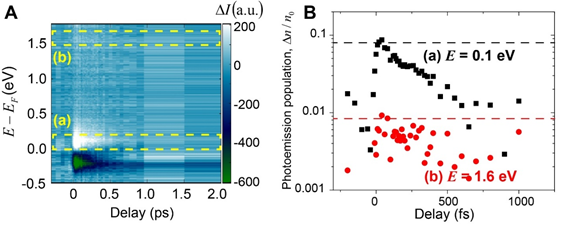
\includegraphics[width=150mm]{figs/NiFigS3}
	\end{center}
	\caption{Electron population dynamics. (A) The relative change of photoemission intensity as a function pump-probe time delay, taking the intensity before pump excitation ($t_d$ = -500 fs) as the reference. The yellow dashed boxes represent the two regions of energy where the changes of electron population are extracted. (B) Normalized electron population as a function of pump-probe time delay extracted from (a) and (b) regions in (A).}
	\label{fig: NiSIfig3}
\end{figure}

\section{Dynamics of Exchange Splitting}

The exchange splitting can be clearly resolved at k$\/\/ \approx 1.05\AA^{-1}$ in the photoemission spectra excited by $\approx$16 eV HHG photons as shown in Fig. \ref{fig: NiSIfig2}C of the main text. In order to extract the exchange splitting and improve the signal to noise ratio in the data analysis, the photoemission intensity is extracted along the direction normal to the band dispersion ($\approx 10\deg$ tilted from the constant momentum direction) as shown in Fig. \ref{fig: NiSIfig4}A and B. The photoemission intensity (I) after Shirley-background subtraction (43) is hence fitted to the function
\begin{equation}
I(E)=\Sigma_{m=1,2,3} A_m \times V(E;E_m^0,\sigma_m^G,\sigma_m^L)
\label{eqn:S2}
\end{equation}
where E is the photoelectron energy, m represents the index of the Voigt functions, $V(E;E_m^0,\sigma_m^G,\sigma_m^L)$ is the normalized Voigt function with $E_m^0$ the center energy,$\sigma_m^G$ the Gaussian width and $\sigma_m^L$ the Lorentzian width of the $m^{th}$ Voigt function, and $A_m$ is the amplitude of the $m^{th}$ Voigt function. The typical fitting results of photoemission intensity are shown in Fig. \ref{fig: NiSIfig4}C-F for fluence below and above $F_{c}$ and at different times. As shown in Fig. \ref{fig: NiSIfig4}C, the first Voigt peak (m=1) represents a low energy d band with a binding energy of $\approx$0.6 eV, which does not change after pump excitation. The second and third Voigt peaks (m=2, 3), on the other hand, correspond to the majority and minority d bands that cross the Fermi energy at k$\/\/ \approx  1.05 \AA^{-1}$(20). When fitting the results to extract the exchange splitting change as a function of pump-probe time delay, we 1) fix the Gaussian width of all Voigt peaks considering the energy resolution of $\approx$160 meV; 2) fix the parameters of the third Voigt function (m=3) and the width of the second Voigt function (m=2), using the values obtained from the ground-state fitting ($t_d$ = -500 fs). As a result, we have 5 fitting parameters $(A_1,E_1^0,\sigma_1^L,A_2,E_2^0)$ and the exchange splitting is defined and extracted as  $E_{ex}=E_1^0-E_2^0$. The extracted $E_{ex}$ is ~240 meV in the ground state, which is consistent with previous works at a similar Brillouin-zone (BZ) point (20). 

\begin{figure}[htbp]
	\begin{center}
		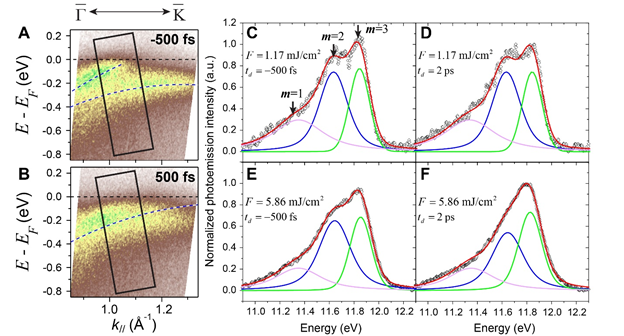
\includegraphics[width=150mm]{figs/NiFigS4}
	\end{center}
	\caption{Analysis of exchange splitting. (A) and (B) Photoemission spectra of Ni(111) before (td = -500 fs) and after (td = 500 fs) pump excitation. The solid black boxes represent the regions the photoemission intensities are extracted for the analysis on the exchange splitting. (C)-(D) The photoemission intensities and the Voigt function fitting (Eq. S2) results for different pump fluences and different pump-probe time delays. The red lines are the overall fitting results. The Cyan, blue and green curves represent the extracted Voigt peaks for m=1, 2 (majority band) and 3(minority band).}
	\label{fig: NiSIfig4}
\end{figure}

We note that our analysis shows that $E_{ex}$ does not vanish after pump excitation. (Same as the sample is heated up across the Curie temperature, see below.) It has been shown that the absolute value of exchange splitting measured in the spin-integrated photoemission depends on the model and the fitting strategy(46). In our work, the 160 meV energy resolution, as well as the fitting model in which two peaks (majority and minority bands) are always assumed to exist, post the limit of our ability to resolve the collapse of the exchange splitting beyond $\Delta E_{ex}$ = 60 meV. In order to extract reliable dynamics of the exchange splitting, we consistently used the same fitting strategy as described above for different time delays as well as different fluences. The fact that the extracted dynamics of exchange splitting can agree with the demagnetization process measured using Tr-TMOKE method (Fig. \ref{fig: Nifig2}A and D) also validates our fitting strategy and strongly suggests that the dynamics of $E_{ex}$ can represent the dynamics of magnetization after pump excitation. At the same time, the difference of exchange splitting for fluence below and above $F_c$ at $t_d$ =  2 ps can be clearly resolved from the raw experimental data as shown in Fig. \ref{fig: NiSIfig4}D and F.

The change of the exchange splitting  ($\Delta E_{ex})$ as a function of $t_d$ under different pump fluence are fit to Eq. 3.2. We find the results can be fit with a set of universal time constants: $\tau_{demag}=176\pm$27 fs, $\tau_{recover_1}$=537$\pm$173 fs and $\tau_{recover_2}$=26$\pm$11 ps, as plotted in Fig. \ref{fig: NiSIfig5}.

\begin{figure}[htbp]
	\begin{center}
		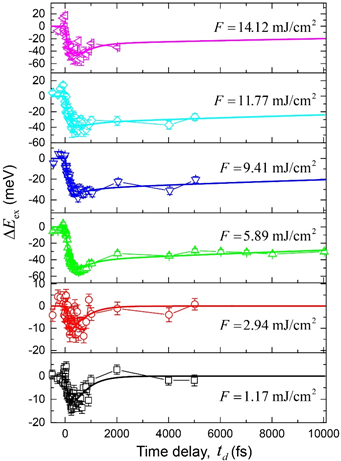
\includegraphics[width=70mm]{figs/NiFigS5}
	\end{center}
	\caption{Global fitting of the exchange splitting dynamics. The global fitting results of the exchange splitting dynamics to Eq. \ref{eqn:2} for a range of pump fluences (F= 1.17 mJ/c$m^2$ to F = 14.12 mJ/c$m^2$).}
	\label{fig: NiSIfig5}
\end{figure}

\section{Temperature dependence of exchange splitting in static ARPES}
The static photoelectron spectrum along  direction measured using He I$\alpha$ photons (h$\nu$ = 21.218 eV) from helium discharge lamp at room temperature is shown in Fig. \ref{fig: NiSIfig6}A. The exchange splitting ($E_{ex}$) between the majority and minority bands of Ni can be clearly observed at the momentum  $\approx$ 1.05 $\AA^{-1}$ where its d band crosses the Fermi energy ($E_F$). The values of $E_{ex}$ can be quantitatively extracted using the same fitting procedures described in the previous section. We find $E_{ex}$ reduces as the sample temperature approaches the Curie temperature (~631 K) as shown in Fig. \ref{fig: NiSIfig6}B, indicating the quenching of the local magnetic moments (1, 20).

\begin{figure}[htbp]
	\begin{center}
		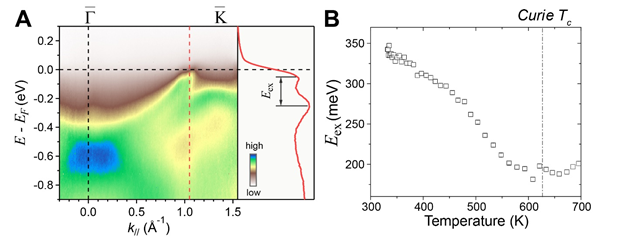
\includegraphics[width=150mm]{figs/NiFigS6}
	\end{center}
	\caption{Collapse of exchange splitting at the Curie temperature. (A) Static photoemission spectrum excited by He I$\alpha$ photons (h$\nu$ = 21.218 eV) at the room temperature. Right panel: Energy distribution curve extracted at the momentum where the red dashed line is located. The exchange splitting ($E_{ex}$) can be clearly extracted using fitting procedure described in the previous section. (B) $E_{ex}$ change reduces as the sample temperature increases.}
	\label{fig: NiSIfig6}
\end{figure}